\documentclass[a4paper,10pt,french]{article}
\usepackage{../../CLT2425}
\geometry{a4paper,tmargin=1cm,bmargin=0.5cm,lmargin=1cm,rmargin=1cm}
%\renewcommand{\familydefault}{\sfdefault}
% \DeclareSymbolFont{numbers}{T1}{cmss}{m}{n}
%%  \SetSymbolFont{numbers}{}{T1}{phv}{bx}{n}
%  \DeclareMathSymbol{0}\mathalpha{numbers}{"30}
%  \DeclareMathSymbol{1}\mathalpha{numbers}{"31}
%  \DeclareMathSymbol{2}\mathalpha{numbers}{"32}
%  \DeclareMathSymbol{3}\mathalpha{numbers}{"33}
%  \DeclareMathSymbol{4}\mathalpha{numbers}{"34}
%  \DeclareMathSymbol{5}\mathalpha{numbers}{"35}
%  \DeclareMathSymbol{6}\mathalpha{numbers}{"36}
%  \DeclareMathSymbol{7}\mathalpha{numbers}{"37}
%  \DeclareMathSymbol{8}\mathalpha{numbers}{"38}
%  \DeclareMathSymbol{9}\mathalpha{numbers}{"39}

\setlength{\columnsep}{30pt}
\begin{document}
\pagestyle{empty}

\titrebis{0.45}{Feuille 4 - Translation et définition}

\bigskip

\begin{multicols}{2}

\textbf{Exercice 1. }
 \`A partir de la figure ci-dessous,
 \begin{enumerate}
  \item donner les images des points $C$, $D$, $E$ dans la translation de vecteur $\V{AB}$;
  \item citer trois vecteurs \'egaux au vecteur $\V{AB}$;
\item citer les trois parall\'elogrammes d\'efinis par les trois \'egalit\'es vectorielles pr\'ec\'edentes.
\end{enumerate}
 \begin{center}
 \begin{tikzpicture}[scale=0.8]
\quadrillageSeyes{(-0.8,-0.8)}{(6.4,4.8)}
\draw [->,epais, color=black] (0.8,3.2) -- (3.2,4);
%\draw  (0.8,3.2) node {$+$};
%\draw  (3.2,4) node {$+$};
\draw  (1.6,1.6) node {$\bullet$};
\draw  (3.2,0.8) node {$\bullet$};
\draw  (0.8,0) node {$\bullet$};
\draw  (4,2.4) node {$\bullet$};
 \draw  (5.6,1.6) node {$\bullet$};
 \draw  (4.8,0.8) node {$\bullet$};
 \draw  (0.8,3.2) node[left] {$A$};
 \draw  (3.2,4) node[above] {$B$};
 \draw  (1.6,1.6) node[left] {$C$};
 \draw  (3.2,0.8) node[left] {$D$};
 \draw  (0.8,0) node[above] {$E$};
  \draw  (4,2.4) node[right] {$Y$};
  \draw  (5.6,1.6) node[left] {$Z$};
 \draw  (4.8,0.8)node[right] {$X$};
 \end{tikzpicture}
\end{center}


\textbf{Exercice 2. }
La figure ci-dessous repr\'esente sept hexagones \\r\'eguliers et num\'erot\'es.
\begin{center}
 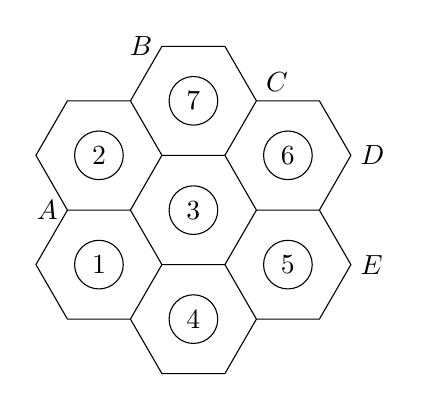
\begin{tikzpicture}[scale=0.4]
\draw [color=black] (2,0)-- (4,0)-- (5,1.73)-- (4,3.46)-- (2,3.46)-- (1,1.73)-- cycle;
\draw[color=black] (3,1.73) node[draw,circle]{1};
\draw [color=black] (4,3.46)-- (5,5.2)-- (4,6.93)-- (2,6.93)-- (1,5.2)-- (2,3.46);
\draw[color=black] (3,5.2) node[draw,circle]{2};
\draw [color=black] (5,1.73) --(7,1.73)-- (8,3.46)-- (7,5.2)-- (5,5.2);
\draw[color=black] (6,3.46) node[draw,circle]{3};
\draw [color=black]   (4,0)-- (5,-1.73)-- (7,-1.73)-- (8,0)--(7,1.73);
\draw[color=black] (6,0) node[draw,circle]{4};
 \draw [color=black]  (8,0)-- (10,0)-- (11,1.73)-- (10,3.46)-- (8,3.46);
\draw[color=black] (9,1.73) node[draw,circle]{5};
 \draw [color=black] (10,3.46)-- (11,5.2)-- (10,6.93)-- (8,6.93)-- (7,5.2);
\draw[color=black] (9,5.2) node[draw,circle]{6};
\draw [color=black] (8,6.93)-- (7,8.66)-- (5,8.66)-- (4,6.93);
\draw[color=black] (6,6.93) node[draw,circle]{7};
\draw (2,3.46) node[left] {$A$};
\draw (5,8.66) node[left] {$B$};
\draw (8,6.93) node[above right] {$C$};
\draw (11,5.2) node[right] {$D$};
\draw (11,1.73) node[right] {$E$};
\end{tikzpicture}
\end{center}
\vspace{-0.5em}
D\'eterminer l'image:
\begin{enumerate}
 \item de l'hexagone 1 dans la translation de vecteur $\V{AC}$;
 \item de l'hexagone 4 dans la translation de vecteur $\V{AB}$;
 \item de l'hexagone 7 dans la translation de vecteur $\V{DE}$.
\end{enumerate}


\end{multicols}

%\Exe{\ \\
% Reproduire la figure puis construire le translat\'e du triangle $ABC$ dans la translation de vecteur $\V{AB}$.
% 
% \begin{center}
% \begin{tikzpicture}[scale=0.8]
%\quadrillageSeyes{(-0.8,0)}{(4,3.2)}
%\draw[fill=gray] (1.6,0.4) -- (3.2,1.2) -- (0,2.4) -- cycle;
%\draw (3.2,1.2) node[above] {$A$};
%\draw (1.6,0.4) node[left] {$B$};
%\draw (0,2.4)  node[left] {$C$};
%\end{tikzpicture}
%\end{center}
%}

\bigskip

\begin{multicols}{2}
\textbf{Exercice 3. }
 \`A partir de la figure ci-dessous, citer un vecteur:
   \begin{enumerate}
    \item oppos\'e \`a $\V{CD}$;
    \item de m\^eme direction et de m\^eme sens que $\V{AC}$;
    \item de m\^eme direction  que $\V{BC}$ mais de sens contraire;
    \item \'egal au vecteur $\V{BA}$.
   \end{enumerate}
   \begin{center}
   \begin{tikzpicture}[scale=0.8]
\quadrillageSeyes{(0,0)}{(8,7.2)}

\pointGraphique{2.4}{3.2}{A}{left}
\pointGraphique{0.8}{0.8}{B}{below}
\pointGraphique{2.4}{0.8}{C}{left}
\pointGraphique{3.2}{1.6}{D}{below}
    \draw[epais, ->, color=black] (0,2.4)--(0.8,2.4);
    \draw[color=black] (0.4,2.4)  node[above] {{\boldmath $\V u$}};
    \draw[epais, ->, color=black] (0.8,4)--(2.4,6.4);
    \draw[color=black] (1.6,5)  node[above left] {{\boldmath $\V v$}};
    \draw[epais, ->, color=black] (3.2,4)--(3.2,5.6);
    \draw[color=black] (3.2,4.8)  node[left] {{\boldmath $\V w$}};
    \draw[epais, ->, color=black] (4,4.8)--(4.8,5.6);
    \draw[color=black] (4.4,5.2)  node[above] {{\boldmath $\V r$}};
    \draw[epais, ->, color=black] (6.4,6.4)--(4.8,2.4);
    \draw[color=black] (5.6,3.6)  node[above] {{\boldmath $\V s$}};
    \draw[epais, ->, color=black] (6.4,6.4)--(5.6,6.4);
    \draw[color=black] (6,6.4)  node[above] {{\boldmath $\V t$}};
    \draw[epais, ->, color=black] (7.2,1.6)--(6.4,0.8);
    \draw[color=black] (6.8,1.2)  node[above] {{\boldmath $\V p$}};
    \draw[epais, ->, color=black] (7.2,4)--(7.2,3.2);
    \draw[color=black] (7.2,3.6)  node[left] {{\boldmath $\V m$}};
   \end{tikzpicture}
   \end{center}
   
   
\textbf{Exercice 4. }
Sur la figure suivante, expliquer, en utilisant les termes direction, sens ou norme, pourquoi le vecteur $\V{AB}$ n'est \'egal \`a aucun des autres vecteurs repr\'esent\'es.\\
\bigskip
\psset{xunit=1cm , yunit=1cm}
\begin{pspicture*}(-0.8,-0.8)(7.7,4.7)
\def\xmin{-0.6} \def\xmax{7.5} \def\ymin{-0.6} \def\ymax{4.5}
\psset{xunit=1cm,yunit=1cm}
\psgrid[griddots=10,gridlabels=0pt,gridwidth=.7pt, gridcolor=black, subgridwidth=.3pt, subgridcolor=black, subgriddiv=1](0,0)(-0.6,-0.6)(7.5,4.5)
\psset{xunit=1cm , yunit=1cm}
\psset{linecolor=black, linewidth=.5pt, arrowsize=2pt 4}
\uput[d](0,2){$A$}
\uput[u](1,3){$B$}
\psline[linewidth=1.4pt]{->}(0,2)(1,3)
\uput[d](1,0){$C$}
\uput[d](3,0){$D$}
\psline[linewidth=1.4pt]{->}(1,0)(3,0)
\uput[d](3,2){$G$}
\uput[u](5,4){$H$}
\psline[linewidth=1.4pt]{->}(3,2)(5,4)
\uput[d](6,1){$E$}
\uput[u](7,2){$F$}
\psline[linewidth=1.4pt]{->}(7,2)(6,1)
\end{pspicture*}

\end{multicols}

\bigskip

\textbf{Exercice 5. }
\begin{multicols}{2}
\begin{small}
On consid\`ere le motif repr\'esent\'e ci-contre.
\begin{enumerate}
	\item Citer tous les vecteurs \'egaux :
		\begin{enumerate}
			\item au vecteur $\V{AB}$ et repr\'esent\'es sur ce motif ;
			\item au vecteur $\V{FE}$ et repr\'esent\'es sur ce motif.
		\end{enumerate}
	\item En n'utilisant que les lettres repr\'esent\'ees sur ce motif, d\'eterminer un vecteur \'egal au vecteur $\V{AB}+\V{FE}$.
	\item En n'utilisant que les lettres repr\'esent\'ees sur ce motif, d\'eterminer un vecteur \'egal aux vecteurs suivants :
		\vspace{-1em}\begin{multicols}{2}\begin{enumerate}
			\item $\V{AB}+\V{AH}$
			\item $\V{BA}+\V{BC}$
			\item $\V{BC}+\V{DE}$
			\item $\V{BF}+\V{GF}$
			\item $\V{AE}+\V{FB}$
			\item[] 
		\end{enumerate}\end{multicols}
\end{enumerate}
\end{small}
\columnbreak
\begin{center}
\psset{xunit=0.75cm,yunit=0.75cm}
\begin{pspicture*}(0.2,0.2)(9.7,7.7)
\def\xmin{0.4} \def\xmax{9.5} \def\ymin{0.4} \def\ymax{7.5}
\psset{xunit=0.75cm,yunit=0.75cm}
\psgrid[gridlabels=0pt,gridwidth=.3pt, gridcolor=gray, subgridwidth=.3pt, subgridcolor=gray, subgriddiv=1](0,0)(0.4,0.4)(9.5,7.5)

\psset{linecolor=black, linewidth=.5pt, arrowsize=2pt 4}
\psdots[dotstyle=+, dotscale=2.0000](3.0000,7.0000)
\psline[linewidth=1.4pt](7,1)(7,5)(9,5)(5,7)(1,7)(1,3)(3,3)(7,1)
\uput[dr](7,1){$A$}
\uput[ul](7,5){$H$}
\uput[r](9,5){$G$}
\uput[u](5,7){$F$}
\uput[u](3,7){$E$}
\uput[ul](1,7){$D$}
\uput[dl](1,3){$C$}
\uput[ur](3,3){$B$}

\end{pspicture*}
\end{center}
\end{multicols}

\end{document}